
\begin{figure}[htb]
   \centering
   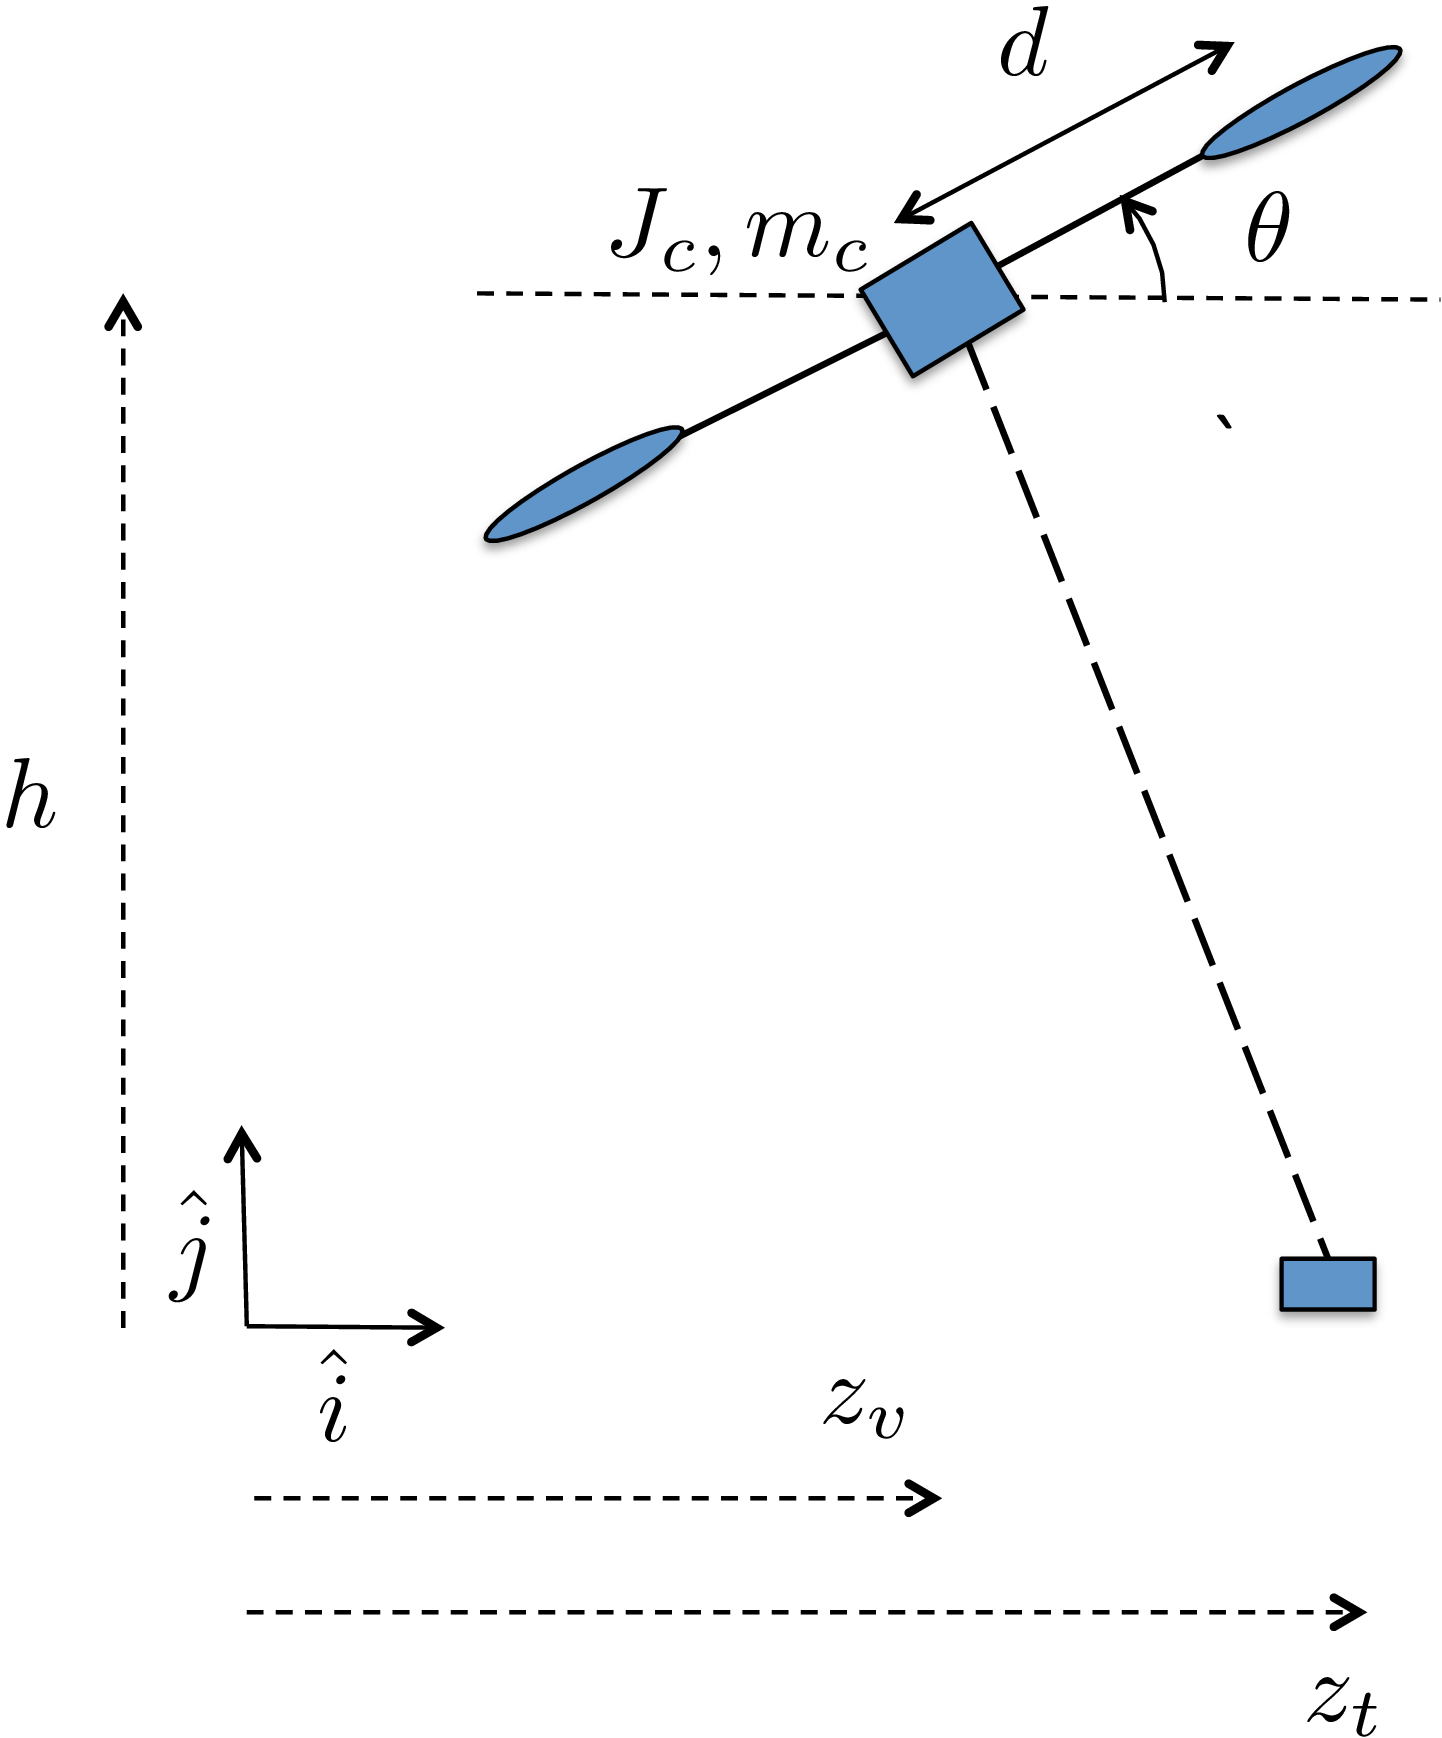
\includegraphics[width=0.5\textwidth]{6_design_studies/figures/hw_planar_VTOL_kinetic_energy} 
   \caption{Computing the kinetic energy for the planar VTOL system.}
   \label{fig:hw_planar_VTOL_kinetic_energy}
\end{figure}


Define the inertial coordinate frame as in Figure~\ref{fig:hw_planar_VTOL_kinetic_energy}, with $\hat{k}$ out of the page.  

There are three masses in the system.  Since the right and left motors are modeled as point masses, they do not have any rotational kinetic energy.  Therefore, the total kinetic energy of the system is given by
\[
K = \frac{1}{2}m_c \mathbf{v}_c^{\top} \mathbf{v}_c + \frac{1}{2}\boldsymbol{\omega}_c^{\top}J_c\boldsymbol{\omega}_c 
+ \frac{1}{2}m_r \mathbf{v}_r^{\top} \mathbf{v}_r 
+ \frac{1}{2}m_\ell \mathbf{v}_\ell^{\top} \mathbf{v}_\ell.
\]
The positions of each mass are given by
\begin{align*}
\mathbf{p}_c &= \begin{pmatrix} z(t) \\ h(t) \\ 0 \end{pmatrix} \\
\mathbf{p}_r &= \begin{pmatrix} z(t)+d\cos\theta(t) \\ h(t) + d\sin\theta(t) \\ 0 \end{pmatrix} \\
\mathbf{p}_\ell &= \begin{pmatrix} z(t)-d\cos\theta(t) \\ h(t)-d\sin\theta(t) \\ 0 \end{pmatrix}.
\end{align*}

Differentiating we obtain
\begin{align*}
\mathbf{v}_c &= \begin{pmatrix} \dot{z} \\ \dot{h} \\ 0 \end{pmatrix} \\
\mathbf{v}_r &= \begin{pmatrix} \dot{z}-d\dot{\theta}\sin\theta \\ \dot{h} + d\dot{\theta}\cos\theta \\ 0 \end{pmatrix} \\
\mathbf{v}_\ell &= \begin{pmatrix} \dot{z}+d\dot{\theta}\sin\theta \\ \dot{h}-d\dot{\theta}\cos\theta \\ 0 \end{pmatrix}.
\end{align*}

The angular velocity of the center pod is given by
\[
\boldsymbol{\omega}_c = \begin{pmatrix} 0 \\ 0 \\ \dot{\theta} \end{pmatrix}.
\]
Therefore, the kinetic energy is given by
\begin{align*}
K &= \frac{1}{2}m_c \left[\dot{z}^2 + \dot{h}^2\right] 
+ \frac{1}{2} J_c \dot{\theta}^2 
\\ &\qquad
+ \frac{1}{2}m_r \left[ (\dot{z}-d\dot{\theta}\sin\theta)^2 + (\dot{h} + d\dot{\theta}\cos\theta)^2 \right] 
\\ &\qquad
+ \frac{1}{2}m_\ell \left[ (\dot{z}+d\dot{\theta}\sin\theta)^2 + (\dot{h}-d\dot{\theta}\cos\theta)^2 \right] 
\\
&= \frac{1}{2} m_c \dot{z}^2 + \frac{1}{2}m_c \dot{h}^2 + \frac{1}{2} J_c \dot{\theta}^2
\\ &\qquad
+ \frac{1}{2}m_r \left[ \dot{z}^2-2d\dot{z}\dot{\theta}\sin\theta + d^2\dot{\theta}^2\sin^2\theta + \dot{h}^2 + 2d\dot{h}\dot{\theta}\cos\theta + d^2\dot{\theta}^2\cos^2\theta \right] 
\\ &\qquad
+ \frac{1}{2}m_\ell \left[ \dot{z}^2+2d\dot{z}\dot{\theta}\sin\theta + d^2\dot{\theta}^2\sin^2\theta + \dot{h}^2 - 2d\dot{h}\dot{\theta}\cos\theta + d^2\dot{\theta}^2\cos^2\theta \right] 
\\
&= \frac{1}{2} (m_c+2m_r) \dot{z}^2 + \frac{1}{2}(m_c+2m_r) \dot{h}^2 + \frac{1}{2} (J_c+2m_rd^2) \dot{\theta}^2,
\end{align*}
where we have used the fact that $m_\ell=m_r$.



